% WR figure exported by sim_ui.py -- 2026-09-18 21:15:58
%
% Preamble (once, in your thesis):
%   \usepackage{pgfplots}
%   \pgfplotsset{compat=1.18}
%
% Use:
%   \begin{figure}[htbp]\centering
%     \input{wr_convergence}
%     \caption{...}\label{fig:...}
%   \end{figure}
%
% \input nests (unlike \include), so this works inside a chapter file the root
% already \includes. Pasting the body below inline works too -- the \definecolor
% lines may then be hoisted into the preamble and dropped from each figure.
%
% Series are thinned to ~2000 points each (min/max decimation, so spikes are
% preserved); edit _PGF_MAX_PTS in sim_ui.py for the full-resolution data.
%
% Run: coupling_mode=voltage-driven; precondition=on (optimized); interface_form=Thevenin (V source); use_t_floor=bare dt; interface_consistency=accumulated; N_field_windows=100; N_xyce_samples=1; xyce_integration_method=Backward-Euler (maxord=1)

\definecolor{C0}{HTML}{1F77B4}
\definecolor{C1}{HTML}{FF7F0E}
\definecolor{C2}{HTML}{2CA02C}
\definecolor{C3}{HTML}{D62728}

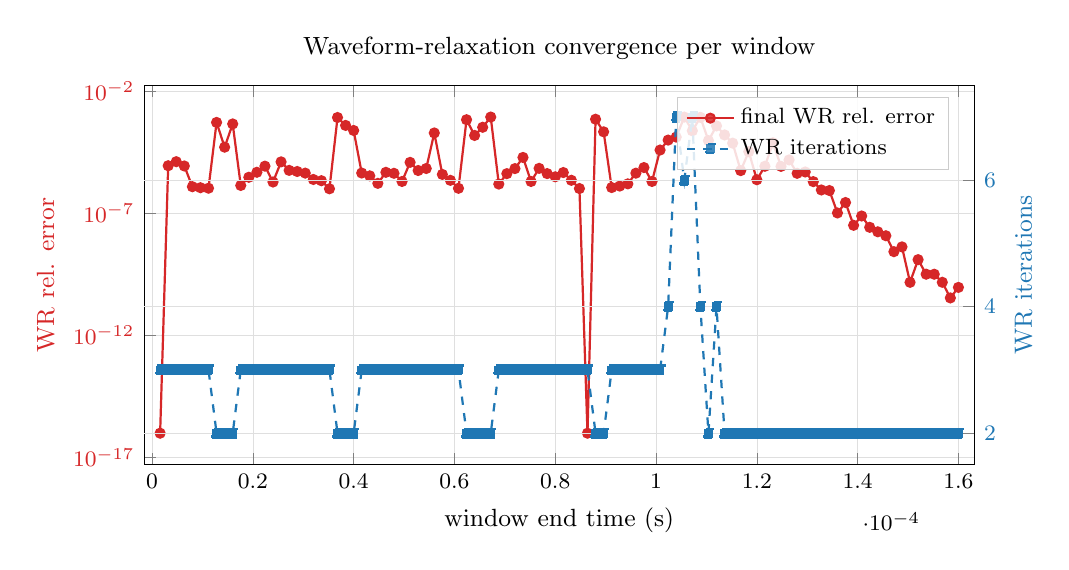
\begin{tikzpicture}
\begin{axis}[
  width=\linewidth,
  height=6.4cm,
  title={Waveform-relaxation convergence per window},
  xlabel={window end time (s)},
  ylabel={WR rel. error},
  grid=both,
  grid style={line width=.2pt, draw=gray!25},
  legend pos=north east,
  legend cell align=left,
  legend style={font=\footnotesize, fill=white, fill opacity=0.85, text opacity=1, draw=gray!40},
  tick label style={font=\footnotesize},
  label style={font=\small},
  title style={font=\small},
  scaled x ticks=true,
  xmin=-1.568e-06,
  xmax=0.000163168,
  ymode=log,
  axis y line*=left,
  ylabel style={color=C3},
  yticklabel style={color=C3}
]
  \addplot[color=C3, line width=0.8pt, mark=*, mark size=1.6pt] coordinates {
    (1.6e-06,1e-16) (3.2e-06,8.804e-06) (4.8e-06,1.288e-05) (6.4e-06,8.598e-06) (8e-06,1.221e-06) (9.6e-06,1.11e-06)
    (1.12e-05,1.059e-06) (1.28e-05,0.0005207) (1.44e-05,5.058e-05) (1.6e-05,0.0004523) (1.76e-05,1.374e-06) (1.92e-05,2.97e-06)
    (2.08e-05,4.75e-06) (2.24e-05,8.455e-06) (2.4e-05,1.9e-06) (2.56e-05,1.267e-05) (2.72e-05,5.686e-06) (2.88e-05,5.116e-06)
    (3.04e-05,4.387e-06) (3.2e-05,2.413e-06) (3.36e-05,2.147e-06) (3.52e-05,1.002e-06) (3.68e-05,0.0008279) (3.84e-05,0.000393)
    (4e-05,0.0002435) (4.16e-05,4.424e-06) (4.32e-05,3.395e-06) (4.48e-05,1.674e-06) (4.64e-05,4.732e-06) (4.8e-05,4.308e-06)
    (4.96e-05,2e-06) (5.12e-05,1.209e-05) (5.28e-05,5.612e-06) (5.44e-05,6.779e-06) (5.6e-05,0.0001932) (5.76e-05,3.881e-06)
    (5.92e-05,2.224e-06) (6.08e-05,1.05e-06) (6.24e-05,0.0006734) (6.4e-05,0.0001528) (6.56e-05,0.0003302) (6.72e-05,0.0008654)
    (6.88e-05,1.565e-06) (7.04e-05,4.18e-06) (7.2e-05,6.719e-06) (7.36e-05,1.925e-05) (7.52e-05,2e-06) (7.68e-05,6.872e-06)
    (7.84e-05,4.199e-06) (8e-05,3.109e-06) (8.16e-05,4.636e-06) (8.32e-05,2.231e-06) (8.48e-05,1.028e-06) (8.64e-05,1e-16)
    (8.8e-05,0.0007046) (8.96e-05,0.0002148) (9.12e-05,1.128e-06) (9.28e-05,1.296e-06) (9.44e-05,1.596e-06) (9.6e-05,4.375e-06)
    (9.76e-05,7.409e-06) (9.92e-05,2e-06) (0.0001008,3.864e-05) (0.0001024,9.86e-05) (0.000104,0.0001307) (0.0001056,0.0008608)
    (0.0001072,0.0002371) (0.0001088,0.0008413) (0.0001104,9.37e-05) (0.000112,0.0003757) (0.0001136,0.0001601) (0.0001152,7.398e-05)
    (0.0001168,5.553e-06) (0.0001184,3.312e-05) (0.00012,2.354e-06) (0.0001216,8.378e-06) (0.0001232,7.626e-05) (0.0001248,8.292e-06)
    (0.0001264,1.524e-05) (0.000128,4.31e-06) (0.0001296,4.888e-06) (0.0001312,1.968e-06) (0.0001328,8.981e-07) (0.0001344,8.506e-07)
    (0.000136,1.029e-07) (0.0001376,2.747e-07) (0.0001392,3.212e-08) (0.0001408,7.724e-08) (0.0001424,2.657e-08) (0.000144,1.742e-08)
    (0.0001456,1.203e-08) (0.0001472,2.682e-09) (0.0001488,4.21e-09) (0.0001504,1.49e-10) (0.000152,1.264e-09) (0.0001536,3.209e-10)
    (0.0001552,3.199e-10) (0.0001568,1.498e-10) (0.0001584,3.426e-11) (0.00016,9.256e-11)
  };
\end{axis}
\begin{axis}[
  width=\linewidth,
  height=6.4cm,
  title={},
  xlabel={},
  ylabel={WR iterations},
  grid=both,
  grid style={line width=.2pt, draw=gray!25},
  legend pos=north east,
  legend cell align=left,
  legend style={font=\footnotesize, fill=white, fill opacity=0.85, text opacity=1, draw=gray!40},
  tick label style={font=\footnotesize},
  label style={font=\small},
  title style={font=\small},
  scaled x ticks=true,
  xmin=-1.568e-06,
  xmax=0.000163168,
  axis y line*=right,
  axis x line=none,
  ylabel style={color=C0},
  yticklabel style={color=C0}
]
  \addlegendimage{color=C3, line width=0.8pt, mark=*, mark size=1.6pt}
  \addlegendentry{final WR rel. error}
  \addplot[color=C0, line width=0.8pt, dashed, mark=square*, mark size=1.6pt] coordinates {
    (1.6e-06,3) (3.2e-06,3) (4.8e-06,3) (6.4e-06,3) (8e-06,3) (9.6e-06,3)
    (1.12e-05,3) (1.28e-05,2) (1.44e-05,2) (1.6e-05,2) (1.76e-05,3) (1.92e-05,3)
    (2.08e-05,3) (2.24e-05,3) (2.4e-05,3) (2.56e-05,3) (2.72e-05,3) (2.88e-05,3)
    (3.04e-05,3) (3.2e-05,3) (3.36e-05,3) (3.52e-05,3) (3.68e-05,2) (3.84e-05,2)
    (4e-05,2) (4.16e-05,3) (4.32e-05,3) (4.48e-05,3) (4.64e-05,3) (4.8e-05,3)
    (4.96e-05,3) (5.12e-05,3) (5.28e-05,3) (5.44e-05,3) (5.6e-05,3) (5.76e-05,3)
    (5.92e-05,3) (6.08e-05,3) (6.24e-05,2) (6.4e-05,2) (6.56e-05,2) (6.72e-05,2)
    (6.88e-05,3) (7.04e-05,3) (7.2e-05,3) (7.36e-05,3) (7.52e-05,3) (7.68e-05,3)
    (7.84e-05,3) (8e-05,3) (8.16e-05,3) (8.32e-05,3) (8.48e-05,3) (8.64e-05,3)
    (8.8e-05,2) (8.96e-05,2) (9.12e-05,3) (9.28e-05,3) (9.44e-05,3) (9.6e-05,3)
    (9.76e-05,3) (9.92e-05,3) (0.0001008,3) (0.0001024,4) (0.000104,7) (0.0001056,6)
    (0.0001072,7) (0.0001088,4) (0.0001104,2) (0.000112,4) (0.0001136,2) (0.0001152,2)
    (0.0001168,2) (0.0001184,2) (0.00012,2) (0.0001216,2) (0.0001232,2) (0.0001248,2)
    (0.0001264,2) (0.000128,2) (0.0001296,2) (0.0001312,2) (0.0001328,2) (0.0001344,2)
    (0.000136,2) (0.0001376,2) (0.0001392,2) (0.0001408,2) (0.0001424,2) (0.000144,2)
    (0.0001456,2) (0.0001472,2) (0.0001488,2) (0.0001504,2) (0.000152,2) (0.0001536,2)
    (0.0001552,2) (0.0001568,2) (0.0001584,2) (0.00016,2)
  };
  \addlegendentry{WR iterations}
\end{axis}
\end{tikzpicture}
